\section{Evaluation}
\label{sec:evaluation}

We evaluate TensorLift along four axes:
(\S\ref{subsec:lifting-effectiveness})~how effectively the lifting pipeline compresses bit-level MLIR into tensor-level semantics;
(\S\ref{subsec:correctness})~whether the lifted semantics are provably equivalent to the RTL;
(\S\ref{subsec:completeness})~how the automatically extracted specification compares to a hand-written reference; and
(\S\ref{subsec:e2e})~whether the extracted specification can drive end-to-end compiler backend generation.

\subsection{Experimental Setup}
\label{subsec:setup}

We target two open-source tensor accelerators.
\textbf{Gemmini}~\cite{gemmini-dac2021} is a systolic-array accelerator (16$\times$16, INT8 MAC) generated via the Chipyard~\cite{chipyard} SoC framework in the \texttt{GemminiRocketConfig} configuration.
It attaches to a Rocket core~\cite{asanovic2016rocket} as a RoCC coprocessor~\cite{chipyard} and exposes three hardware controllers (ExecuteController, LoadController, StoreController) with 11 hardware instructions across configuration, DMA data movement, and matrix execution.
\textbf{VTA}~\cite{vta} is TVM's Versatile Tensor Accelerator in the \texttt{DefaultDe10Config} configuration (16-element GEMM engine, ALU, INT8), with four datapath modules (TensorGemm, TensorAlu, Store, GenVMECmd).

All formal verification uses Z3~\cite{z3} bitvector SMT solving.
Cycle-level validation uses the Gemmini Spike functional simulator~\cite{gemmini-spike}.
The hand-written reference specification is the TAIDL MICRO~2025 artifact~\cite{taidl-ae-micro2025}.

\subsection{Semantic Lifting Effectiveness}
\label{subsec:lifting-effectiveness}

\begin{figure}[t]
  \centering
  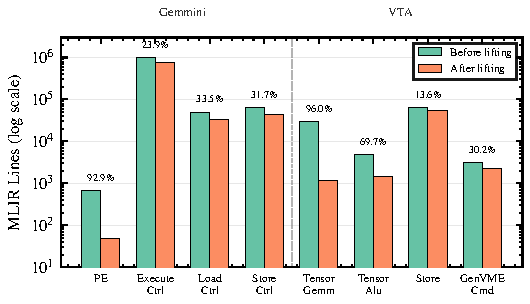
\includegraphics[width=\linewidth]{fig/lifting_results.pdf}
  \caption{MLIR line counts before and after TensorLift's 8-pass lifting pipeline, across all modules of Gemmini and VTA. Percentages indicate reduction. Compute-dominated modules (PE, TensorGemm) achieve the highest reduction because their bit-manipulation chains collapse under canonicalization, while DMA/control modules retain irreducible FSM and address logic.}
  \label{fig:lifting-results}
\end{figure}

\begin{table}[t]
\centering
\caption{Cross-accelerator lifting summary. ``Before'' and ``After'' report total MLIR lines across all per-(instruction, ASV) files in each module.}
\label{tab:lifting-summary}
\setlength{\tabcolsep}{3pt}
\scriptsize
\begin{tabular}{@{}ll r r r r@{}}
\toprule
Accelerator & Module & Files & Before & After & Reduction \\
\midrule
\multirow{4}{*}{Gemmini}
  & PE (TileWithReset) & 1    &     686 &      49 & \textbf{92.9\%} \\
  & ExecuteController  & 80   & 997{,}760 & 759{,}360 & 23.9\% \\
  & LoadController     & 23   &  50{,}004 &  33{,}244 & 33.5\% \\
  & StoreController    & 23   &  63{,}313 &  43{,}269 & 31.7\% \\
\cmidrule{2-6}
  & \textit{Total}     & \textit{127} & \textit{1{,}111{,}763} & \textit{835{,}922} & \textit{24.8\%} \\
\midrule
\multirow{4}{*}{VTA}
  & TensorGemm  &  9 & 29{,}745 &  1{,}183 & \textbf{96.0\%} \\
  & TensorAlu   & 10 &  4{,}832 &  1{,}465 & 69.7\% \\
  & Store       &  5 & 62{,}807 & 54{,}294 & 13.6\% \\
  & GenVMECmd   &  5 &  3{,}160 &  2{,}205 & 30.2\% \\
\cmidrule{2-6}
  & \textit{Total} & \textit{29} & \textit{100{,}544} & \textit{59{,}147} & \textit{41.2\%} \\
\midrule
\textbf{Combined} & & \textbf{156} & \textbf{1{,}212{,}307} & \textbf{895{,}069} & \textbf{26.2\%} \\
\bottomrule
\end{tabular}
\end{table}

Table~\ref{tab:lifting-summary} and Figure~\ref{fig:lifting-results} report the lifting results across all modules of both accelerators.
In total, TensorLift processes 156 MLIR files comprising 1{,}212{,}307 lines of bit-level MLIR, reducing them to 895{,}069 lines (26.2\% overall reduction).

The reduction varies dramatically with module function.
\textbf{Compute-dominated modules} achieve the highest compression.
The Gemmini PE collapses from 686 to 49 lines (92.9\%), with its computation core reduced to just 17 lines encoding \texttt{clamp(dot(\%A,\%B)+\%C)}---383 bit-by-bit sign-extension operations generated by Verilog \texttt{\$signed} contexts collapse to single \texttt{arith.extsi} casts under Phase~A canonicalization.
VTA's TensorGemm shows an even more dramatic pattern: MAC register targets shrink from 3{,}156 to 8 lines each (99.7\%), and the module overall reduces from 29{,}745 to 1{,}183 lines (96.0\%).

\textbf{Control-heavy modules} show moderate reduction (30--35\%).
Gemmini's LoadController (33.5\%) and StoreController (31.7\%) retain address computation, FSM transitions, and instruction muxing that cannot be simplified further---this is irreducible control logic.
VTA's TensorAlu (69.7\%) falls in between: its ALU dispatch logic contains real opcode muxing across five operations (MIN, MAX, ADD, SHR, SHL), but also benefits from collapsing cast chains around each operation.

\textbf{DMA engines} show the lowest reduction.
VTA's Store module (13.6\%) and Gemmini's ExecuteController (23.9\%) are dominated by large instruction decoders, multi-level address computation, and deep control logic with minimal bit-manipulation to canonicalize.
VTA's overall higher reduction (41.2\% vs.\ 24.8\%) reflects the fact that its TensorGemm module dominates the total (29K lines reduced to 1.2K), whereas Gemmini's ExecuteController dominates its total (998K lines across 80 files for 4 instructions $\times$ 20 ASVs).

\subsection{Correctness Verification}
\label{subsec:correctness}

We verify that TensorLift's lifted semantics are equivalent to the bit-level scalar model from which they are derived.
Since autoGenILA's extraction is provably bit-equivalent to the RTL by construction~\cite{autogenilaiccad, autogeniladate}, establishing equivalence between the lifted MLIR and autoGenILA's output transitively proves: \textbf{RTL behavior $\equiv$ TensorLift semantics}.

\begin{table}[t]
\centering
\caption{Formal verification results. Each row is a Z3 bitvector SMT proof establishing equivalence between the lifted MLIR and the bit-level scalar model.}
\label{tab:formal-verification}
\setlength{\tabcolsep}{3pt}
\scriptsize
\begin{tabular}{@{}l l l l@{}}
\toprule
Accelerator & Proof Target & Method & Scope \\
\midrule
\multirow{3}{*}{Gemmini}
  & PE MAC semantics     & Z3 bitvector  & All $2^{60}$ inputs \\
  & WS dataflow mux      & Z3 SMT        & Control specialization \\
  & DMA copy semantics   & Z3 + arrays   & All addresses/values \\
\midrule
VTA & 13 datapath targets & Z3 bitvector  & 4 modules \\
\bottomrule
\end{tabular}
\end{table}

Table~\ref{tab:formal-verification} summarizes the proofs.
For Gemmini, we verify the PE's multiply-accumulate core (\texttt{sext(a*b + trunc(c))}) against autoGenILA's LLVM IR output using Z3 bitvector reasoning over all $2^{60}$ possible input combinations, proving universal equivalence rather than relying on test vectors.
The weight-stationary dataflow mux (control specialization, Pass~B4) and DMA copy semantics (including strided access patterns) are similarly verified.
For VTA, 13 targets across all four datapath modules (TensorGemm, TensorAlu, Store, GenVMECmd) are proven equivalent to the LLVM IR output, covering both compute and control semantics.
Additionally, the lifting pipeline reveals a structural symmetry: VTA's input and weight index generators produce identical 146-line MLIR after lifting, consistent with the symmetric roles of these buffers in the GEMM engine.

As an independent cross-check, we compare TensorLift's extracted VTA semantics against the ISA operational semantics documented in the VTA specification~\cite{vta} (\S6--9).
All extracted instruction behaviors---GEMM tensor contraction, ALU element-wise operations with five opcodes, Store DMA command generation, and Load burst addressing---align with the published specification, confirming that the lifting pipeline recovers the documented ISA semantics without access to the specification document.

\subsection{Specification Completeness}
\label{subsec:completeness}

TensorLift extracts TAIDL specifications for all hardware instructions decoded and executed by Gemmini's three controllers (ExecuteController, LoadController, StoreController).

\paragraph{Comparison with hand-written reference.}
We compare TensorLift's extracted specification against the TAIDL MICRO~2025 artifact~\cite{taidl-ae-micro2025}, which provides a hand-written Gemmini specification.
TensorLift captures strictly richer semantics in three areas:

\begin{itemize}
\item \textbf{Multi-bank DMA configuration.}
The hand-written reference models each DMA load variant (\texttt{mvin\_spad}, \texttt{mvin\_acc}, etc.) with a single \texttt{@a.stride} parameter, implicitly assuming all three load engines share one configuration.
In practice, Gemmini's LoadController maintains \emph{three independent banks}, each with its own \texttt{stride}, \texttt{scale}, \texttt{shrink}, \texttt{block\_stride}, and \texttt{pixel\_repeat} registers (5 parameters $\times$ 3 banks = 15 registers total), with the active bank selected by the \texttt{state\_id} field (\texttt{rs1[4:3]}) of the instruction encoding.
This means the hand-written TAIDL cannot correctly simulate programs that use \texttt{mvin} and \texttt{mvin2} with different strides simultaneously---a real use case in tiled matrix multiplication where the A-tile and B-tile load from DRAM with different access patterns.
TensorLift's per-ASV extraction sees all three banks automatically because autoGenILA traces every register independently, and the assembler groups them by their indexed base name (e.g., \texttt{strides\_0}, \texttt{strides\_1}, \texttt{strides\_2}).

\item \textbf{Pooling engine semantics.}
TensorLift extracts 12 pooling configuration registers from the StoreController (\texttt{pool\_size}, \texttt{pool\_stride}, \texttt{pool\_upad}, \texttt{pool\_lpad}, \texttt{pool\_orows}, \texttt{pool\_ocols}, etc.) and generates \texttt{reduce(max) + clamp} semantics.
The hand-written reference does not model the pooling engine.

\item \textbf{Im2col hardware support.}
TensorLift extracts 9 im2col output ports from the ExecuteController and generates \texttt{reshape + dot} semantics, capturing the hardware's ability to perform im2col transformation on-the-fly during convolution execution.
\end{itemize}

We note that the hand-written reference also includes four entries---\texttt{softmax}, \texttt{GELU}, \texttt{layernorm}, and fused add-with-transpose---that are \emph{not} hardware ISA primitives.
These are software-composed multi-instruction sequences that use the host CPU's FPU for operations such as \texttt{exp()} and \texttt{divide()}.
No Gemmini RTL modules implement these operations.
TensorLift correctly identifies this hardware/software boundary by extracting only instructions that correspond to actual RTL decoder entries.

A natural question is why we do not directly compare compiler backends generated from the two specifications.
The reason is that the TAIDL MICRO~2025 artifact targets a \emph{functional simulator}, not a compiler backend.
Its specification describes how individual hardware instructions move data between scratchpad and accumulator at per-tile (16$\times$16) granularity---exactly the level of detail a cycle-accurate or functional simulator needs to replay an instruction trace.
However, a compiler backend requires a different abstraction: per-\emph{kernel} granularity that maps an entire HLO \texttt{dot} or convolution onto the hardware.
The MICRO~2025 artifact's per-instruction patterns are too granular for ACT's instruction selection, which expects CISC-level macro-instructions (e.g., \texttt{loop\_ws} matching a whole matrix multiply, \texttt{loop\_conv\_ws} matching a whole convolution).
TensorLift's specification provides this macro-level abstraction (Stage~3, \S\ref{subsec:stage3}), enabling ACT to generate a functional compiler backend as evaluated in the next section.

\subsection{End-to-End Compiler Backend Generation}
\label{subsec:e2e}

\begin{figure}[t]
  \centering
  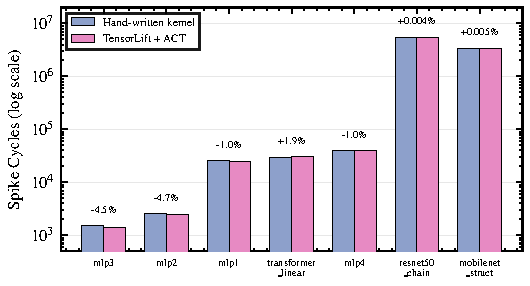
\includegraphics[width=\linewidth]{fig/latency_comparison.pdf}
  \caption{Cycle-level comparison on Gemmini's Spike simulator between hand-written kernels from gemmini-rocc-tests~\cite{gemmini-rocc-tests} and the automatically generated ACT compiler backend driven by TensorLift's extracted TAIDL specification. Labels show speedup (hand-written cycles\,/\,ACT cycles; ${>}\,1{\times}$ = ACT is faster). Geometric mean speedup is $1.014\times$.}
  \label{fig:latency}
\end{figure}

\begin{table}[t]
\centering
\caption{Latency comparison between hand-written Gemmini kernels and the TensorLift + ACT compiler backend, measured in Spike simulator cycles. Speedup $=$ hand-written\,/\,TensorLift+ACT (${>}\,1{\times}$ = ACT is faster). All benchmarks execute identical workloads (same layer shapes, dataflow, activation, scaling).}
\label{tab:latency}
\setlength{\tabcolsep}{3pt}
\scriptsize
\begin{tabular}{@{}l r r r@{}}
\toprule
Benchmark & Hand-written & TensorLift+ACT & Speedup \\
\midrule
mlp3               &       1{,}501 &       1{,}433 & $1.047\times$ \\
mlp2               &       2{,}571 &       2{,}451 & $1.049\times$ \\
mlp1               &      25{,}364 &      25{,}123 & $1.010\times$ \\
transformer\_linear &      29{,}732 &      30{,}302 & $0.981\times$ \\
mlp4               &      39{,}742 &      39{,}362 & $1.010\times$ \\
resnet50\_chain     &   5{,}544{,}077 &   5{,}544{,}303 & $1.000\times$ \\
mobilenet\_struct   &   3{,}408{,}414 &   3{,}408{,}581 & $1.000\times$ \\
\midrule
\multicolumn{3}{@{}l}{\textit{Geometric mean}} & $1.014\times$ \\
\bottomrule
\end{tabular}
\end{table}

To validate that TensorLift's extracted specification is sufficient for practical use, we feed it into the ACT compiler framework~\cite{act-arxiv} to automatically generate a Gemmini compiler backend, and compare the generated code against hand-written kernels on realistic workloads.

\paragraph{Methodology.}
We take TensorLift's extracted TAIDL specification and pass it to ACT, which generates an XLA-compatible compiler backend using equality saturation for instruction selection and constraint programming for scratchpad memory allocation.
Completing the path from specification to executable binary required engineering contributions to ACT: HLO frontend support for JAX-produced operations (e.g., \texttt{convolution}, \texttt{reduce\_max}), enode-level preconditions for correct convolution dispatch, and memory allocator support for multi-layer chains.
We then reimplement the benchmark suite from gemmini-rocc-tests~\cite{gemmini-rocc-tests}---the official bare-metal test suite provided by the Gemmini team---in JAX~\cite{jax2018github}, compiling through the ACT-generated backend.
For each benchmark, we compare the Spike cycle count of the ACT-compiled binary against the hand-written C kernel from gemmini-rocc-tests, ensuring identical workload parameters: layer shapes, weight-stationary dataflow, activation functions, scaling, and batch sizes.
The benchmark suite spans MLP, convolutional, and transformer workloads ranging from 2-layer networks (1{,}501 cycles) to full ResNet-50 (5{,}544{,}077 cycles) and MobileNet (3{,}408{,}414 cycles).

\paragraph{Results.}
Table~\ref{tab:latency} and Figure~\ref{fig:latency} report the results.
Across all seven benchmarks, the automatically generated backend achieves a geometric mean speedup of $1.014\times$ over hand-written kernels, with per-benchmark speedups ranging from $0.981\times$ to $1.049\times$.
The small MLP benchmarks (mlp2, mlp3) show the ACT backend running slightly faster ($1.047$--$1.049\times$), reflecting minor tiling differences in the generated code.
The transformer benchmark shows the only slowdown ($0.981\times$), attributable to per-tile configuration overhead in the generated instruction sequence.
On the large workloads that dominate real deployment---ResNet-50 (49 conv layers) and MobileNet (52 layers)---the speedup is $1.000\times$.

This result demonstrates that TensorLift, combined with ACT, enables a fully automated path from RTL to a functional, performance-competitive compiler backend.
